\documentclass[10pt]{beamer}
\usepackage[english]{babel}
\usepackage{graphicx}
\usepackage{pgfkeys}
\usepackage{tikz}
\usepackage{amstext}
\usetheme{Boadilla}
\title[The SDHCAL technological proposal]{The SDHCAL technological proposal \\ Construction, first results and ongoing R\&D}
\author{L. Mirabito}
\institute{IPN Lyon, UCB Lyon, IN2P3, CNRS}
\date{November 11, 2014}

\begin{document}
% \AtBeginSection[]
% {
%   \begin{frame}<beamer>
%     \frametitle{Plan}
%     \tableofcontents[currentsection,currentsubsection]
%   \end{frame}
% }

\setbeamerfont{frametitle}{size=\huge,series=\bfseries}

\begin{frame}
  \titlepage
\end{frame}

\section{Introduction}
\begin{frame}[shrink=5]{Introduction}


  \begin{columns}
    \begin{column}{0.6\textwidth}
      \begin{block}{\small Context}
   	{\small The SDHCAL-GRPC is one of the two HCAL options proposed
          in the ILD Letter Of Intention (LOI). Modules are  made of 
          48 RPC chambers (6$\lambda_I$) equipped with 
          power-pulsed electronics readout.}   
      \end{block}
      
      \begin{block}{ \small SDHCAL-ILD}
        {\small The structure proposed for the SDHCAL-ILD :
          \par $ ~ \rightarrow$ Is self-supporting 
          \par $ ~\rightarrow$ Has negligible dead zones 
          \par $ ~ \rightarrow$ Eliminates projective cracks 
          \par $ ~ \rightarrow$ Minimizes barrel / endcap separation 
        }
      \end{block}

      \begin{block}{\small  Challenges}
        {\small 
          \par $ ~ \rightarrow$ Thickness of only few mms
          \par $ ~ \rightarrow$ Homogeneity for large surfaces
          \par $ ~ \rightarrow$ Services from one side
          \par $ ~ \rightarrow$ Embedded power-pulsed electronics
          \par $ ~ \rightarrow$ Self-supporting mechanical structure 
          
        }
      \end{block}

    \end{column}

    \begin{column}{0.45\textwidth}
      \centerline{\includegraphics[width=0.45\textwidth]{images/IldDhcal}}
      \centerline{\includegraphics[width=0.55\textwidth]{images/DHCALProtoSchema}}
    \end{column}
  \end{columns}
\end{frame}

\begin{frame}{Detector Choice}

  \begin{block}{Glass Resistive Plate Chamber}
    \begin{columns}
      \begin{column}{0.5\textwidth}
        {
   	  \par $ ~ \rightarrow$ Thin, homogeneous, cost-effective
          \par $ ~ \rightarrow$ High granularity achievable
        }   
      \end{column}
      \begin{column}{0.5\textwidth}
        \centerline{\includegraphics[width=0.9\textwidth]{images/ShowerExample}}
      \end{column}
    \end{columns}
  \end{block}
  
  \pause   

  \begin{block}{  Semi Digital}
    \begin{columns}
      \begin{column}{0.5\textwidth}
        {
          \par $ ~ \rightarrow$ Saturation on 1 $cm^2$ pad in the core of hadronic showers 
          \par $ ~\rightarrow$ 2-bits semi-digital readout improves resolution
        }
      \end{column}

      \begin{column}{0.5\textwidth}
        \centerline{\includegraphics[width=0.9\textwidth]{images/DigitalSemiDigital}}
      \end{column}
    \end{columns}

  \end{block} 

\end{frame}

\begin{frame}{GRPC design}

  \centerline{\includegraphics[width=0.9\textwidth,height=0.4\textheight]{images/GRPCSchema}}
  \pause   

 \begin{columns}
      \begin{column}{0.45\textwidth}
       \centerline{\includegraphics[width=0.9\textwidth]{images/GasFlow}}
      \end{column}
\pause
      \begin{column}{0.45\textwidth}

       \centerline{\includegraphics[width=0.9\textwidth]{images/CoatingStudies}}
      \end{column}
    \end{columns}
  

\end{frame}
\begin{frame}[shrink=3]{Readout Electronic}
\begin{block}{HardRoc asic}
    \begin{columns}
      \begin{column}{0.5\textwidth}
        {\small 
          \par $ ~ \rightarrow$ 64 channels, triggerless mode, 127 memory slots
          \par $ ~\rightarrow$  3 thresholds [10 fC,  15 pC]
          \par $ ~\rightarrow$  Channel gain : Uniformity correction
          \par $ ~\rightarrow$  Analog power switch: Power-pulsed capability, low consumption

        }
      \end{column}

      \begin{column}{0.5\textwidth}
         \centerline{\includegraphics[width=0.9\textwidth]{images/HR2Chip}}
         \centerline{\includegraphics[width=0.9\textwidth]{images/HR2GainAdjustement}}
      \end{column}

    \end{columns}
\end{block}
\pause
\begin{block}{ASU PCB devlopment}
    \begin{columns}
      \begin{column}{0.5\textwidth}
        {\small 
          \par $ ~ \rightarrow$ 8-Layers, buried vias, 50 x 33 cms
          \par $ ~\rightarrow$  Two 24 asics PCB connected with flat connectors
          \par $ ~\rightarrow$  DAQ board (DIF) controls and read the 48 daisy chained chips
        }
      \end{column}

      \begin{column}{0.5\textwidth}
         \centerline{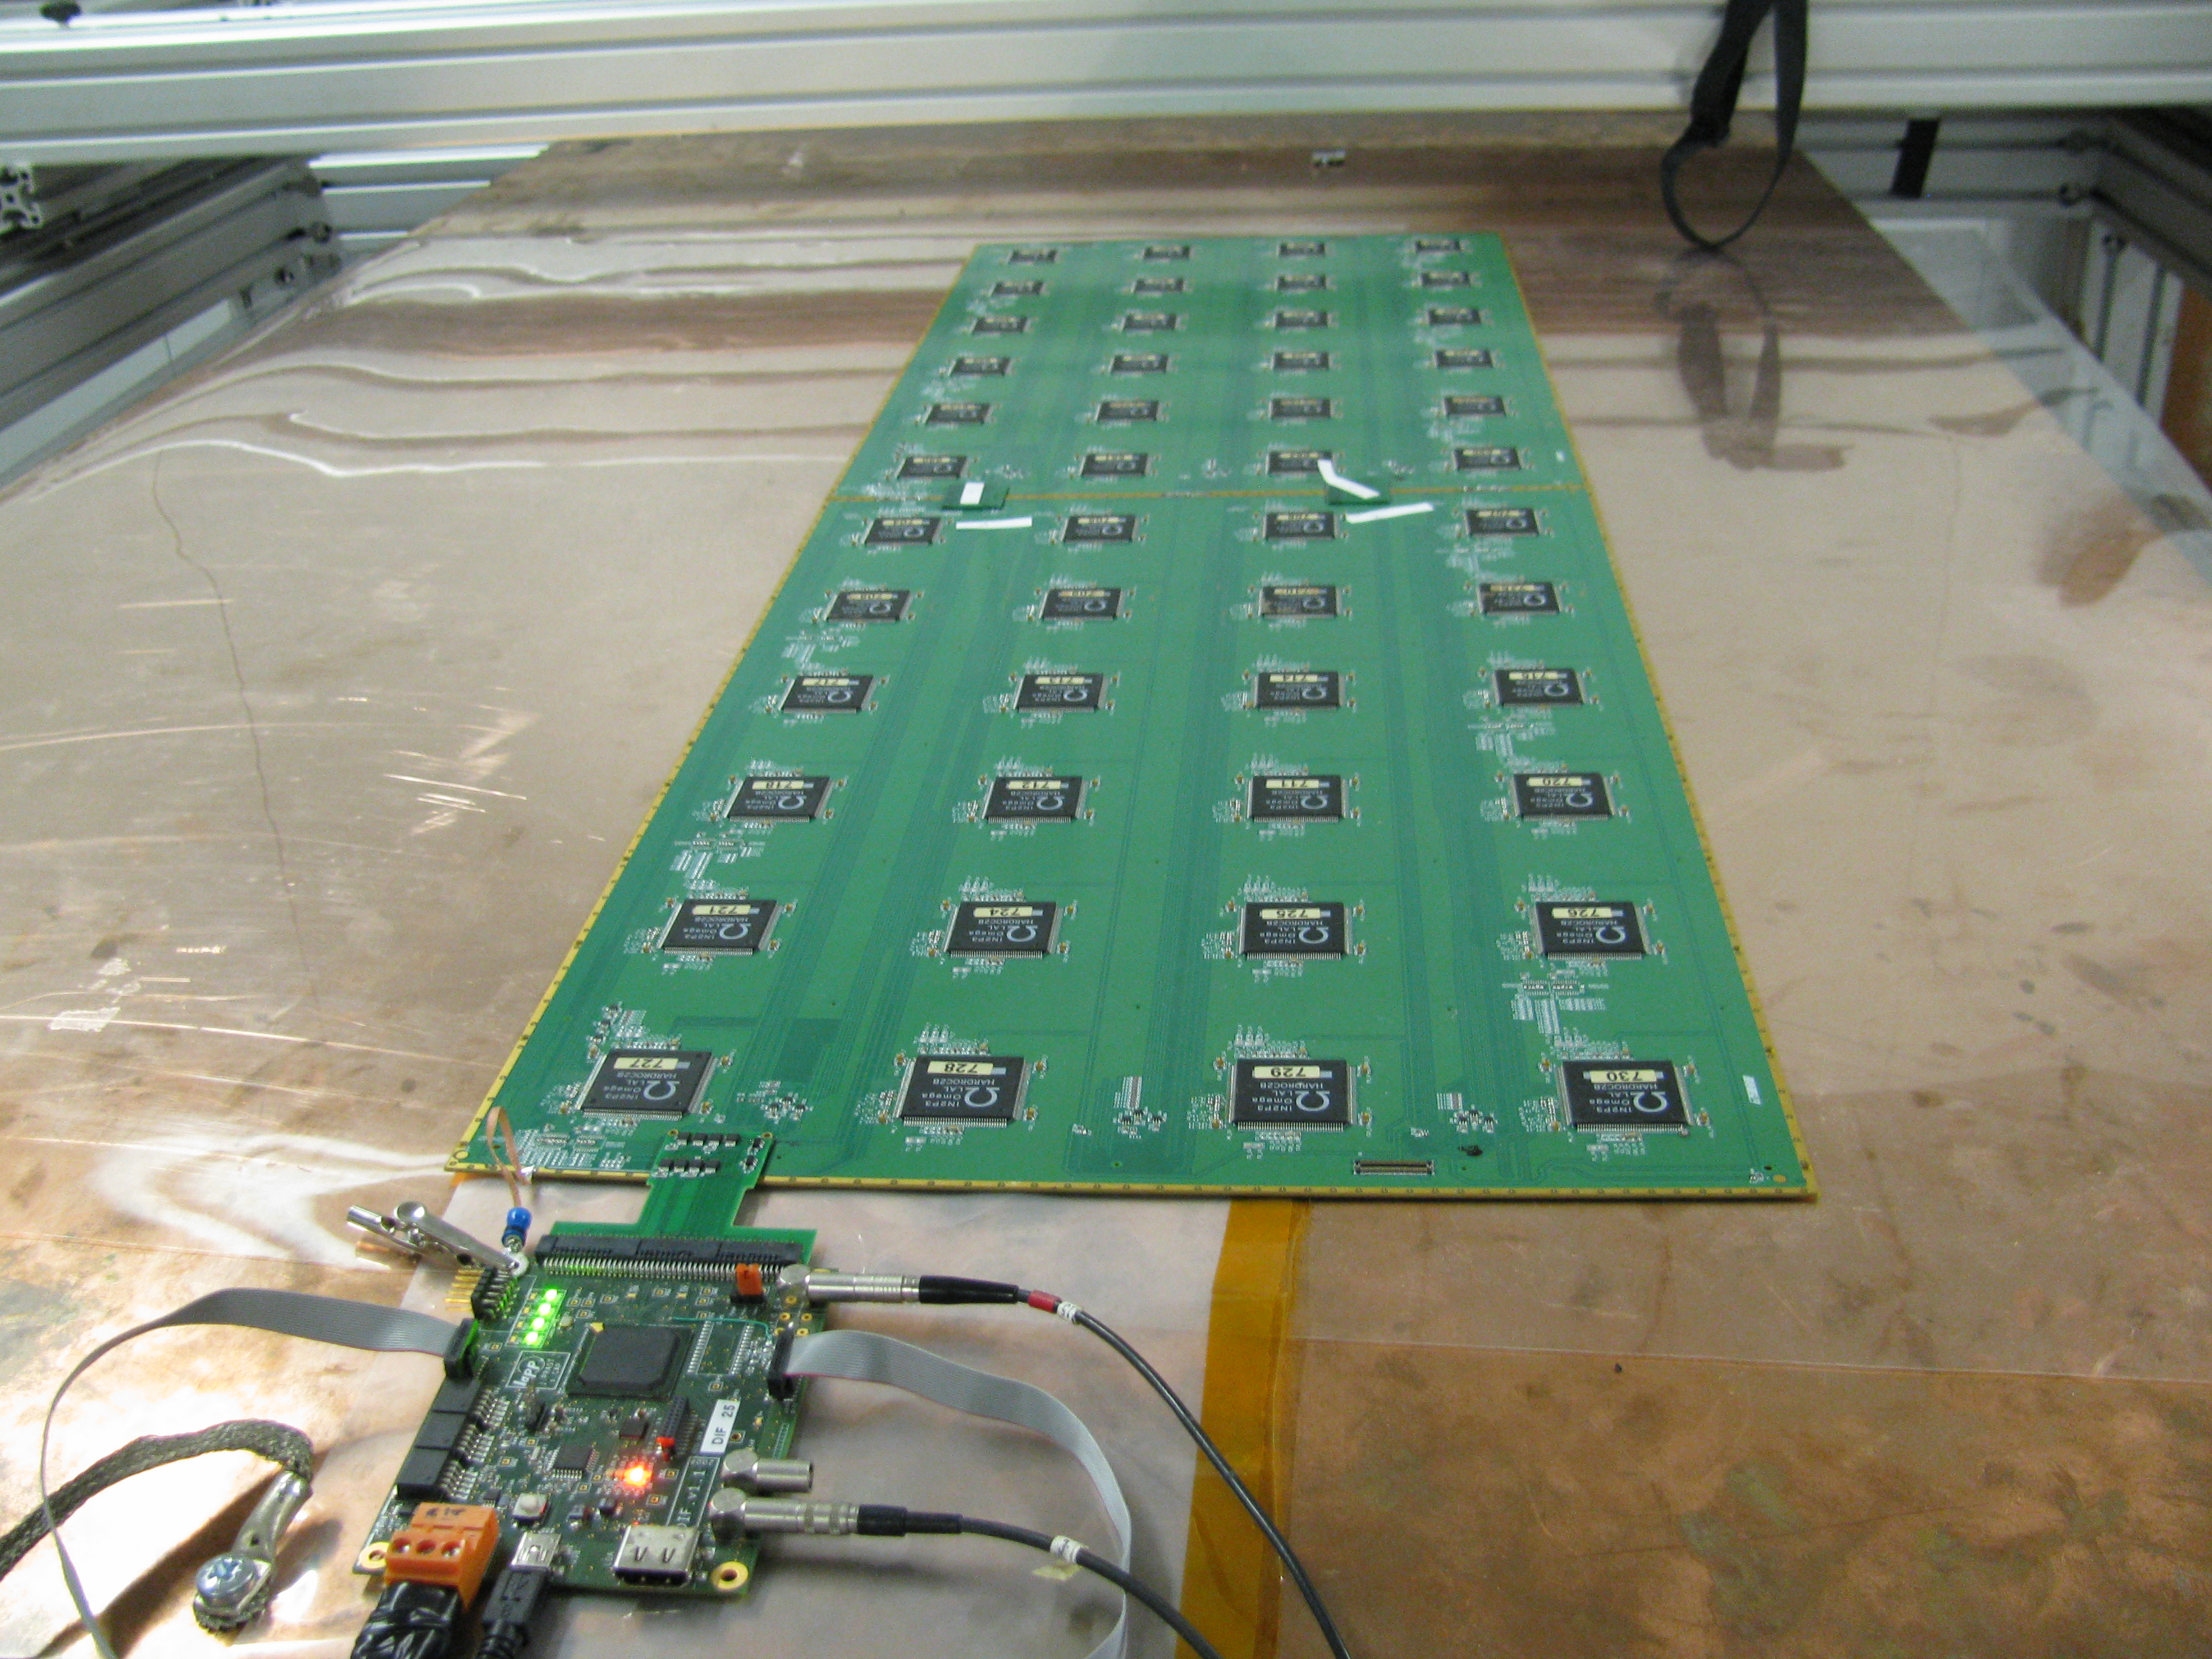
\includegraphics[width=0.9\textwidth]{images/DIFAsu}}
      \end{column}

    \end{columns}
\end{block}
\end{frame}
\begin{frame}{Cassette assembly}
\begin{columns}
      \begin{column}{0.5\textwidth}

        \centerline{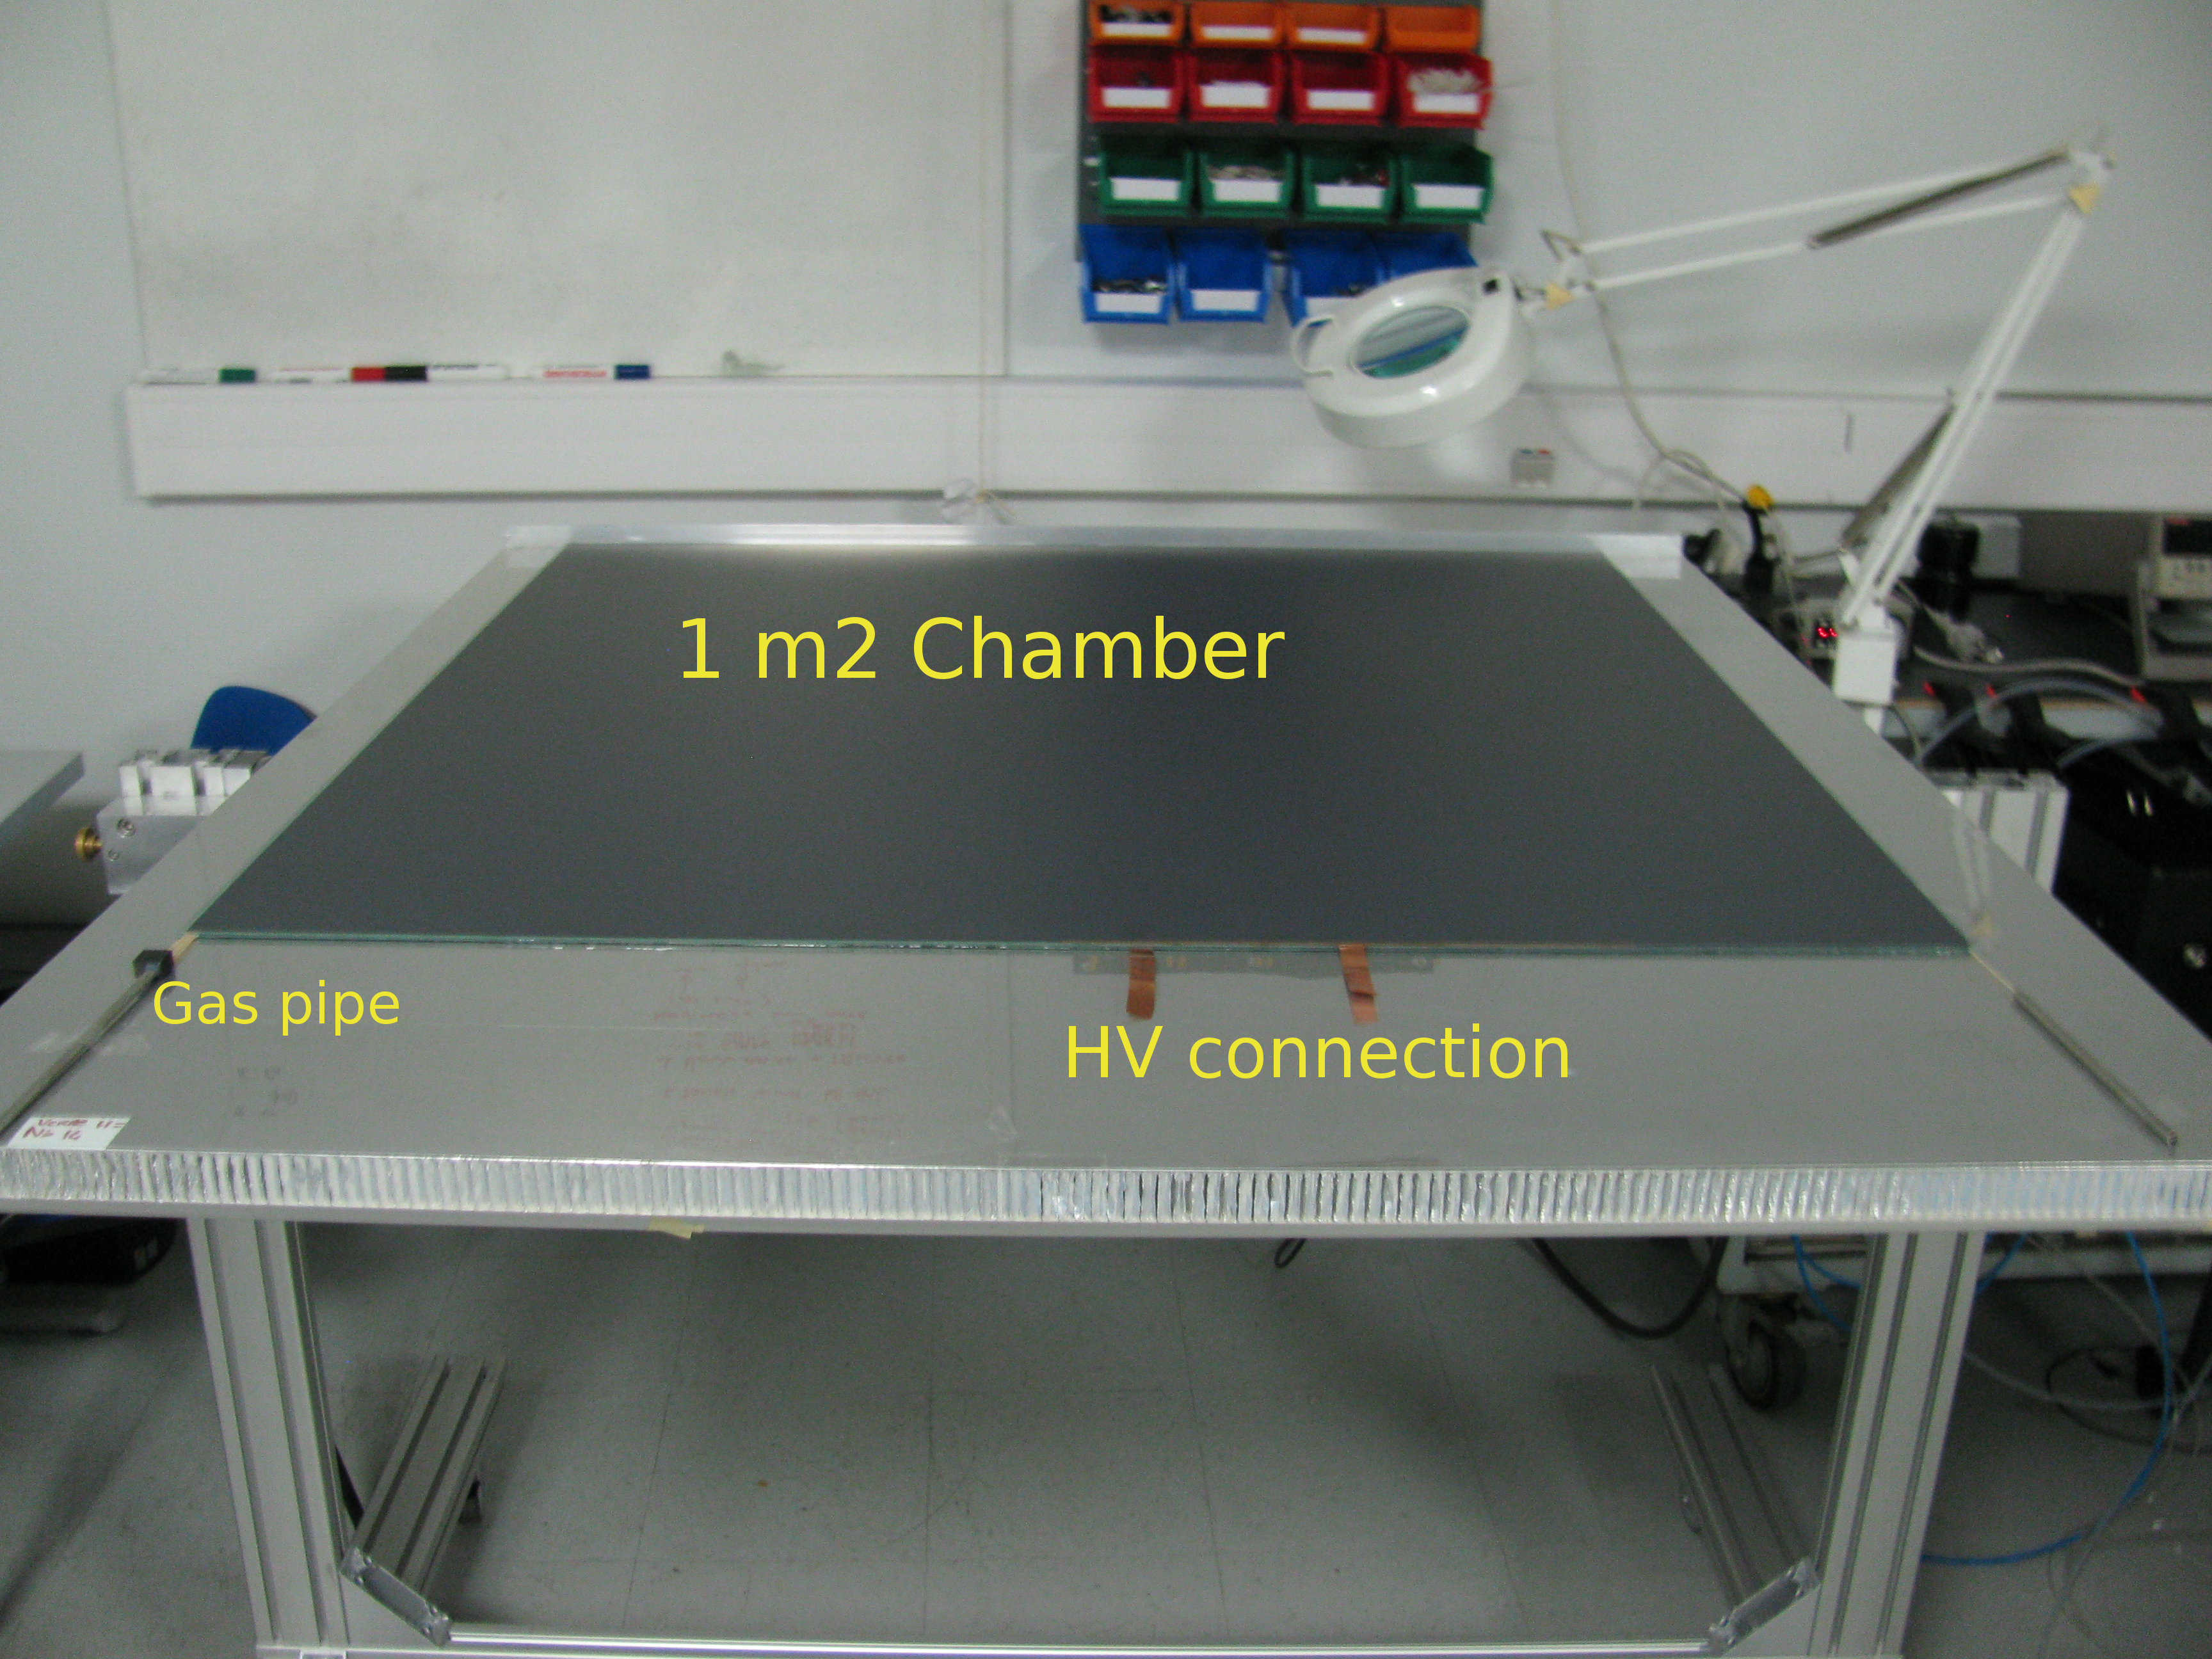
\includegraphics[width=0.9\textwidth]{images/ConstructionRPC}}
      \end{column}
\pause
      \begin{column}{0.5\textwidth}


        \centerline{\includegraphics[width=0.9\textwidth]{images/1m2HR2}}
      \end{column}
    \end{columns}
\begin{columns}
\pause

      \begin{column}{0.5\textwidth}

         \centerline{\includegraphics[width=0.9\textwidth]{images/1m2Cover}}
      \end{column}
\pause
      \begin{column}{0.5\textwidth}

        
        \centerline{\includegraphics[width=0.9\textwidth]{images/1m2Cassette}}
      \end{column}
    \end{columns}

\end{frame}
\begin{frame}{Acquisition system}
 \centerline{\includegraphics[width=0.9\textwidth,height=0.45\textheight]{images/DAQLinks.png}}
 \begin{block}
   {\small 
          \par $ ~\rightarrow$  Oracle configuration data base
          \par $ ~\rightarrow$  Event building with CMS Event Event builder (XDAQ)
          \par $ ~ \rightarrow$ Up to 150 USB links on 4 PCs
          \par $ ~\rightarrow$  Rate limited by USB1 links and daisy chaining 


        }
 \end{block}
\end{frame}
\begin{frame}{Chamber performances  }
\begin{block}{ Cosmic muons studies}
  \begin{columns}

      \begin{column}{0.5\textwidth}
        \centerline{\includegraphics[width=0.9\textwidth]{images/LocalEfficiency}}
      \end{column}
      \begin{column}{0.5\textwidth}
        \centerline{\includegraphics[width=0.9\textwidth]{images/LocalMultiplicity}}
      \end{column}
    \end{columns}
\end{block}

\end{frame}
\begin{frame}{Chamber performances  }
\begin{block}{Power-pulsed performances in 3T B field (H2-CERN)}
 \begin{columns}

      \begin{column}{0.5\textwidth}
        \centerline{\includegraphics[width=0.9\textwidth]{images/PowerPulsingPhoto}}
      \end{column}
     
      \begin{column}{0.5\textwidth}
        \centerline{\includegraphics[width=0.9\textwidth]{images/PowerPulsingHvScan}}
%        \centerline{\includegraphics[width=0.9\textwidth]{images/CoatingStudies}}
      \end{column}
    \end{columns}
\end{block}

\end{frame}


\end{document}
